%%%%%%%%%%%% FORMATO DE LA REVISTA MOMENTO %%%%%%%%%%%%%%%%%

% The files must be in the same working folder: moment (LaTeX Class type), article (LaTeX Class type), these files should not be modified. It must also contain Bibfile files (BibTex Database type) where the author must enter the reference data in BibTex and Format.tex formats (in this file the content of the document is edited)
\documentclass{momento}
\usepackage[pdftex]{graphicx}
\usepackage[spanish,activeacute]{babel}
\usepackage[latin1]{inputenc}
\usepackage{verbatim}
\usepackage[centerlast,sc,footnotesize]{caption2}
\usepackage{subfigure}
\usepackage{amsmath}
\usepackage{amssymb}
\usepackage[mathscr]{euscript}
\usepackage[none]{hyphenat}
\usepackage{multirow}
\usepackage{soul}
\renewcommand{\captionlabeldelim}{.}
\newcommand{\comillas}[1]{``#1"}

\setlength{\parindent}{0pt}

%%%%%%%%%%% TITULO DEL ARTICULO (Los títulos, resúmenes y palabras clave se organizan dependiendo del idioma en el que se escriba el artículo. Entonces, si el artículo se escribe en español se debe colocar primero el título en español y luego en inglés. Si el artículo se escribe en inglés se coloca primero el título en inglés y luego en español. Así mismo para el resumen y palabras clave)
\title{ Optical properties of iridescent minerals\\[0.5cm]
Propiedades opticas de los minerales iridiscentes}

%%%%%%%%%%% AUTHORS
\author{Stephanie Carolina Cely Rodriguez\suprm1, Rafael Rey Gonzalez \suprm2 }
% Por cada autor \suprm# es para referenciar la afiliacion del autor con el número #. Se debe incluir de cada autor el primer nombre, inicial del segundo nombre si lo tiene y el primer apellido. 

%%%%%%%%%%% Affiliation author 
\newcommand{\afiliacion}{\suprm 1 \suprmUniversidad Nacional de Colombia (Grupo de Fotonica, Departamento de Física, Universidad Nacional de Colombia, Bogotá, Colombia) I }


%%%%%%%%%%% Page headers
\newcommand{\autor}{Author I and Author II}
\newcommand{\tema}{Optical properties of iridescent minerals}


%%%%%%%%%%%E-MAIL
\authorinfo{Name of the corresponding author: eccelyr@unal.edu.co}


%%%%%%%%%%% PAGE IN WHICH THE ARTICLE BEGINS (RESERVED FOR THE EDITOR)
\setcounter{page}{1}

% 
\bibliographystyle{apsrev4-1}
\begin{document}
\begin{sloppypar}
  \maketitle


%%%%%%%%%%% ABSTRACT OF YOUR ARTICLE IN ENGLISH
\begin{ingles}
In 1966  Bolton et al. made measurements of the spectral distribution of light reflected by Labradorite, along with TEM observations, in order to find the origin of its color. They proposed a lamellar model for the iridescence properties seen in certain minerals, due to optical interference. 
Previous research has been done on such called labradorescence effect by Weidlich and Wilkie, intended to improve the predictive rendering technique based on reflectance model.
As Joannopoulos and E. Yablonovitch predicted photonic crystals, it has been shown that nature exhibits dependence of shape and geometry to produce structural color, and its understanding may lead to solve technological challenges in material science.
In this study, we analyze the orientation dependent optical response of rocks samples where iridescence can be found.
Samples were polished and then photographed both by regular camera and Petrographic microscope to reveal internal fractures and nanostructures. 
In particular, light reflectance on the mineral's surface was measured through monochromatic laser spectra towards find a relation to the photonic crystal approach.
\end{ingles}
%%%%%%%%%%% keywords
\ikeywords{Keywords written in English.}

%%%%%%%%%%% ABSTRACT OF YOUR ARTICLE IN SPANISH 
\begin{resumen}
Escribir resumen en español
\end{resumen}

%%%%%%%%%%% keywords
\keywords{Palabras clave en español.}

%%%%%%%%%%% BODY OF THE DOCUMENT

\subsection*{Introduction}

Comienzo del cuerpo del artículo.\\

Works to be published must include the generally accepted structure for articles in scientific magazines, with the basic elements:
\begin{itemize}
\item \textbf{Title of the article}. Must be in Spanish and English, in capital letters, without formulas or abbreviations. It must be precise and coherent with the subject in question and must not exceed 150 characters, including blanks. Titles, abstracts and keywords are set up depending on the language the article is written in. So, if the article is written in Spanish, the title must first be written in Spanish and then in English. If the article is written in English the title goes first in English, then in Spanish. Likewise for Abstracts and keywords.\vspace{-0.2cm}
\item \textbf{Authors names}. The given name, initial of the second name if any, and first family name must be included, for each author. List the authors’ filiations with super-indexes, and the contact author’s email (only one) with whom the magazine will exchange correspondence. \vspace{-0.2cm}
\item \textbf{Abstracts in Spanish and English}. 250 words maximum. It must contain the main objective, the most important findings and the conclusions of the research work. \vspace{-0.2cm}
\item \textbf{Keywords}. 5 words maximum. Utilize specific or disciplinary thesaurus in accordance to the subject of the document and not included in the title of the paper. \vspace{-0.2cm}
\item\textbf{Development of the article}. The text must be divided in sections, each one with a headline. i. e. Introduction, Experimental Part and/or Theoretical Development, Results and Discussion, Conclusions. Titles must be left aligned and highlighted in bold. It is recommended that these sections be brief and well balanced.
 \vspace{-0.2cm}
\item\textbf{Bibliographic References}. Only references appearing in the bibliography must be quoted and must be numbered consecutively (as they appear) in square parenthesis. No references can be quoted in the abstract. Bibliographic References must follow the American Physical Society format (Use of BibTEX is recommended) The Magazines’ titles must be abbreviated unless they are not included in the Journal Title Abbreviations or in http://www.ncbi.nlm.nih.gov/nlmcatalog/journals.   In general, quotes must include: Family name and initials of given name of all authors, separated by comas, followed by the Magazine’s name, year, volume and pages. If the publication has DOI, it must be included. For files written in Microsoft Word, insert after the year, if possible, the Web address or link for each quoted reference. (Use of the Endnote tool is suggested) The citations included in this document are examples on how quoting should be done: An article  \cite{1}, a book \cite{2}, a thesis  \cite{3}, proceedings of a congress \cite{4}, unpublished material  \cite{5} and web pages  \cite{6}.Unpublished material refers to papers accepted for publication but not yet printed. \vspace{-0.2cm}
\end{itemize}

\subsubsection*{Requirements}

- Figures and tables must be consecutively numbered and must include in the lower part a title or explanatory text. Figures must have good resolution (at least 300 ppi), must be sent separately in format jpg, pgn, tif or gif, in gray’s scale or in color if strictly necessary. When plotting different data, use when possible different symbols (data markers in Excel), as shown in fig. \ref{figura1}. The physical copies will be printed in black and white but in the web page the articles will present the figures in color.

\begin{figure}[!ht]
\begin{center}
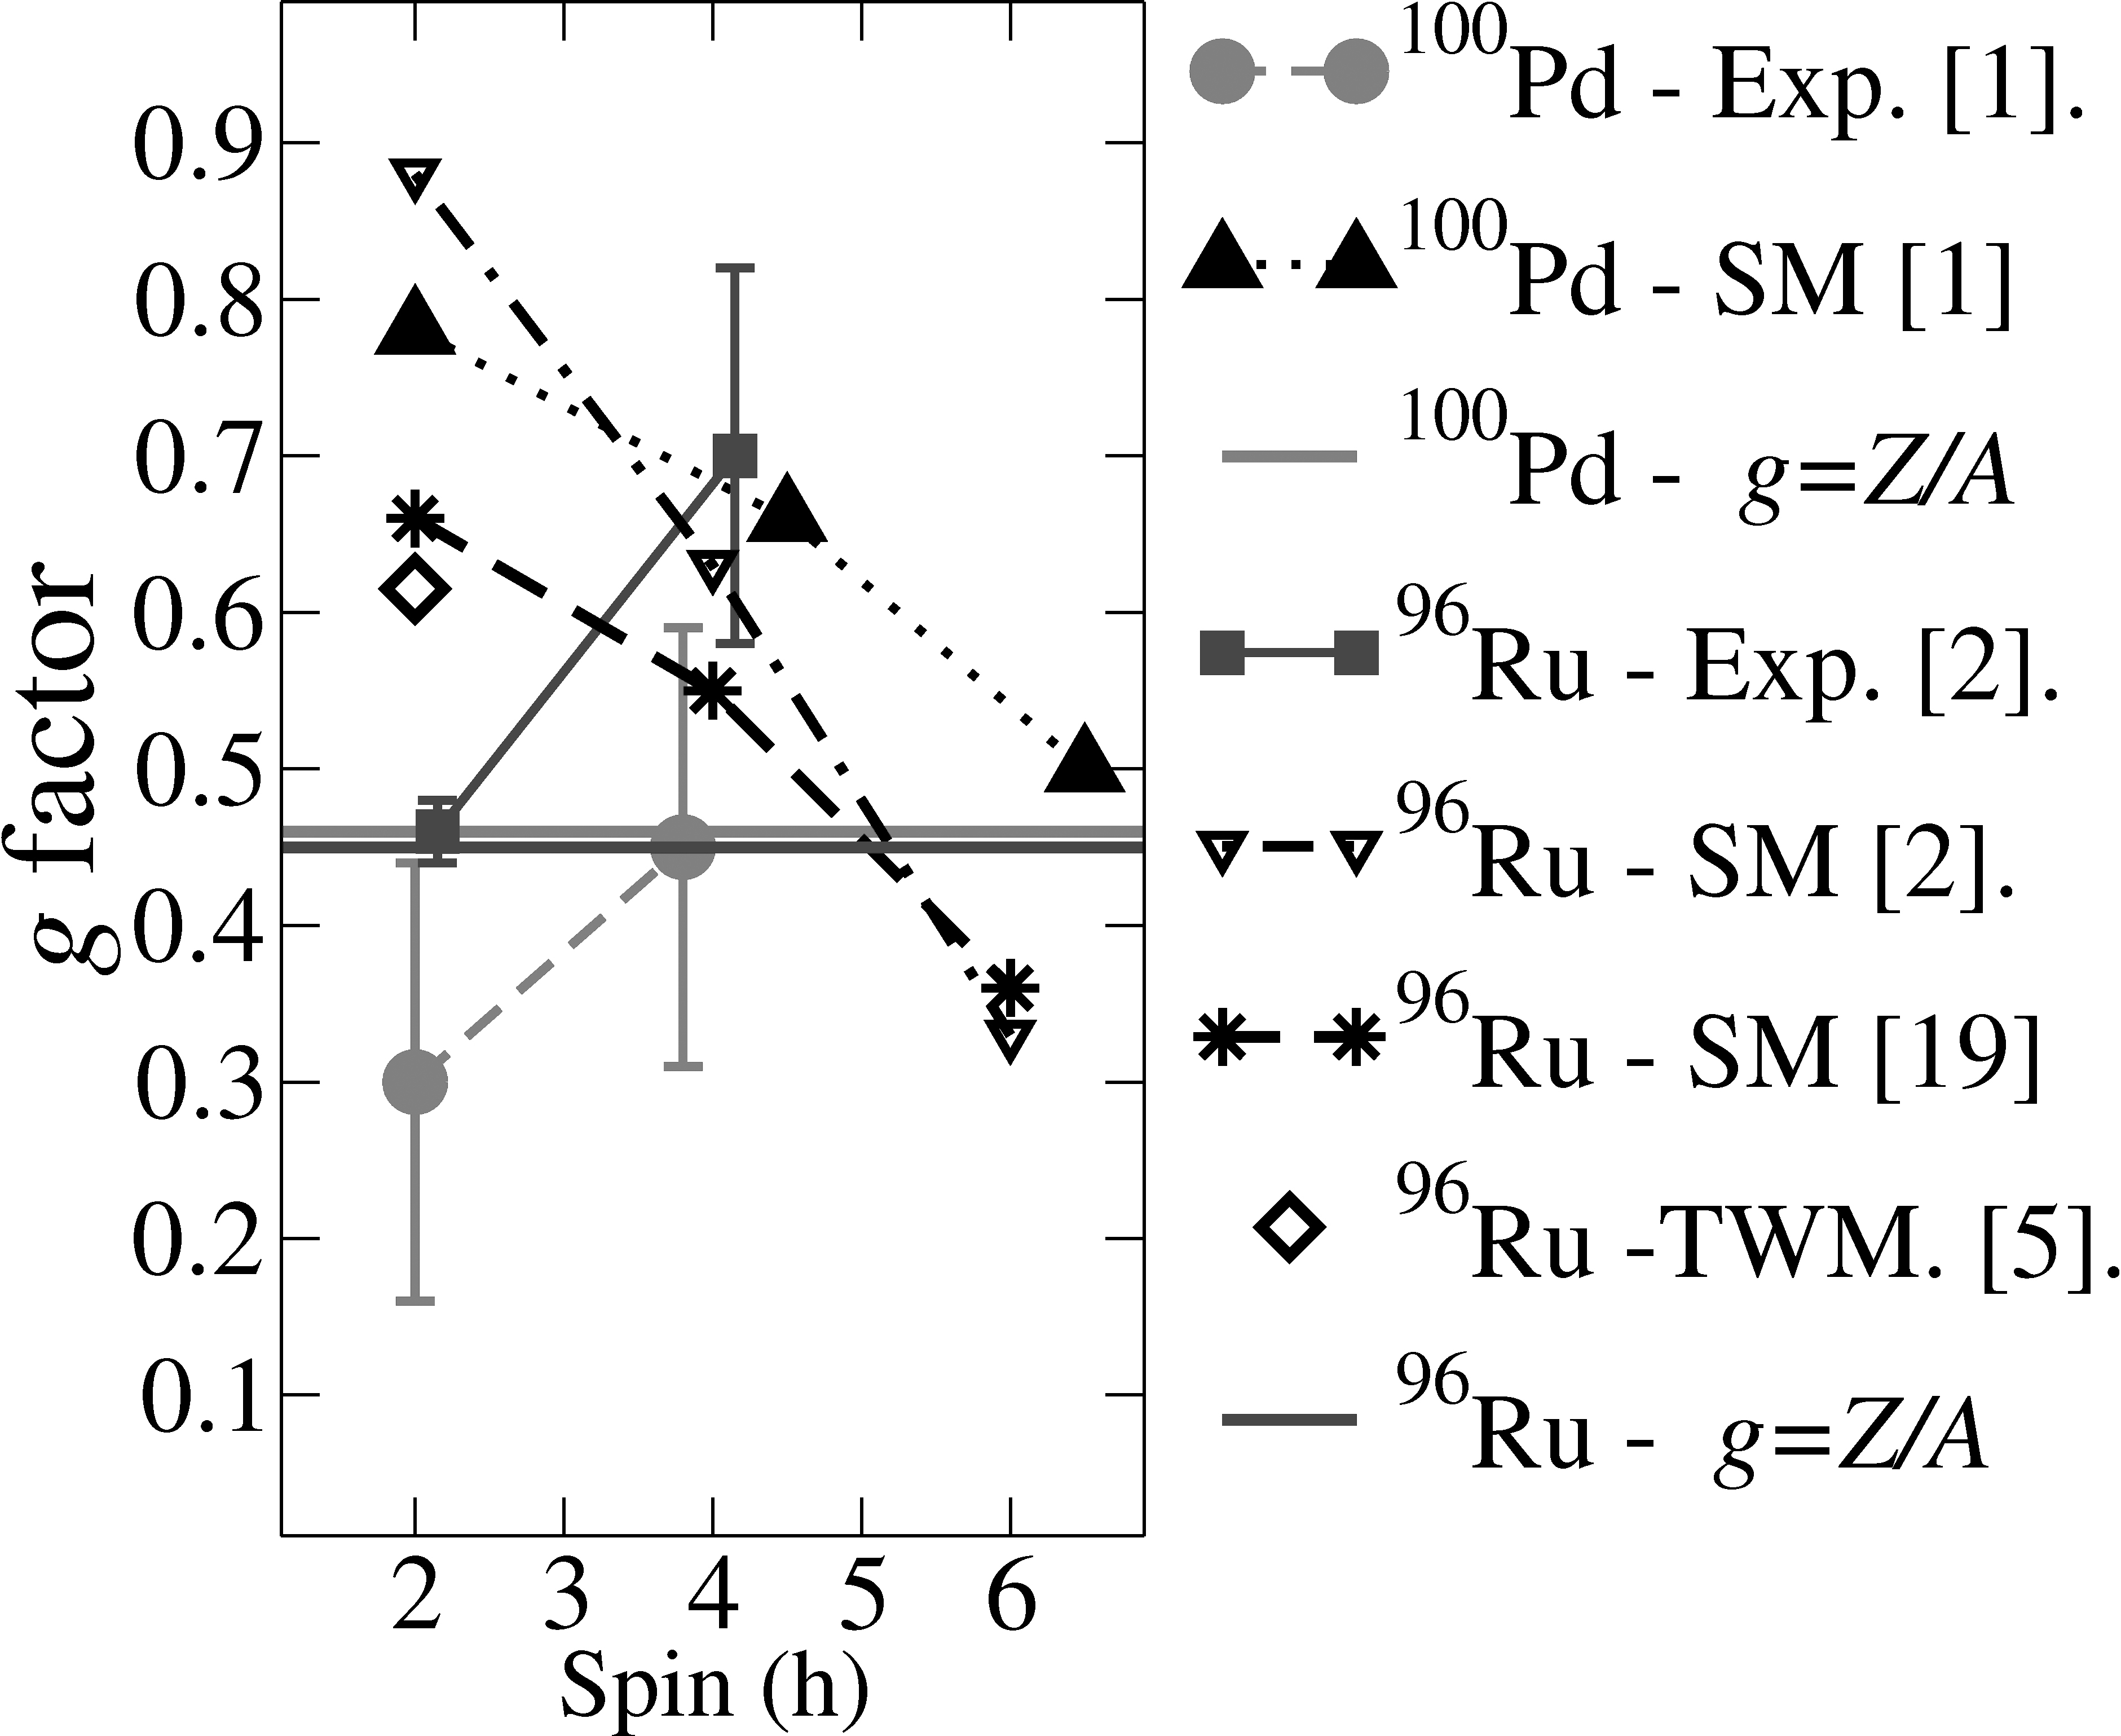
\includegraphics[width=7cm]{figura1.jpg}
\end{center} \vspace{-0.3cm}
\caption{\itshape Example of figure.}  
\label{figura1}
\end{figure}

- \textit{Units, abbreviations and symbols}: The International System of Units is mandatory (m, kg, s, K), using only terms generally accepted. It is necessary to explain the unknown abbreviations when used for the first time. Special care must be exercised when writing symbols in order to make them clearly identifiable with the author, use of formulas, special characters etc.\\

- If gratitude, acknowledgements to entities, publication permits etc are required, they will be at the end of the text and before the bibliographic references\\

- It is recommended to reduce the number of footnotes, especially those quoting other footnotes from the same document and not to use them to mention bibliographic references.\\

- Single line spacing (1.0) must be used for the entire document. However, after each subtitle double spacing is recommended.\\

- The information to this template, i.e. keep page size, margins, letter type (Times New Roman), size, alignment (depending on if it is title, subtitle, table or graph title) and further specifications presented in this template.\\

- An additional requirement is to fill out forms ``\textbf {Originality declaration, authorship responsibility and conflict of interests}'' and ``\textbf {copyright transfer form}'' and send them via email or attach them as complementary files in the OJS system.\\

- Contributions must not exceed 20 pages..


\subsection*{Conclusions}
Conclusions of the article.


\bibliography{bibfile}
\end{sloppypar}
\end{document}



